% !TEX root = ../main.tex
\chapter{Elektrisitet}
\label{Chapter:elektrisitet}

\intro{Dette er en introtekst, hvor vi henviser til\cite{OleBrumm} for mer informasjon. Dette er altså en flott tekst som fungerer som et slags sammendrag / motivasjon for innholdet i kapitlet.}

\spm{}{%
\item Hva er elektrisk ladning og elektrisk strøm?
\item Hva er sammenhengen mellom spenning, strøm og motstand (Ohms lov)?
\item Hvordan fungerer serie- og parallellkoblinger i en krets?}
\newpage

\section{Begreper}
Her kommer noen begreper som er relevante å forstå for dette kapittelet.

\textbf{Elektrisitet}\\
Elektrisitet er små partikler med positive eller negative ladninger.\\


\textbf{Krets}\\
En krets er en vei som strømmen går igjennom. Strømmen går alltid gjennom den delen av kretsen som er lukket. Gjennpm en åpen krets går det ingen strøm. Elektronene i en krets beveger seg motsatt retning som strømmen. Elektronene vil bevege seg fra en negativ ladd pol mot en positiv ladd pol. \\


\textbf{Elektrisk strøm}\\
Elektrisk strøm er partikler i bevegelse. Strøm har symbolet \textit{I} og enhet ampere, [A]. Strømmen beveger seg fra den positive polen mot den negative polen. \\
Strømmen i en krets kan illustreres slik: \\

\begin{figure}[H]
    \centering
    
\includegraphics[width=0.1\linewidth]{Images/Kapittel6:Elektrisitet/Strøm_illustrering.png}
    \caption{Caption}
    \label{fig:enter-label}
\end{figure}


\textbf{Spenning}\\
Tenk på spenning som et «elektrisk høydekart»: akkurat som en ball ruller ned fra høyt til lavt i tyngdefeltet,
beveger ladninger seg fra høyt spenningspotensial til lavt.

\defn{Spenning}{%
Spenningen $U$ mellom to punkter er arbeidet som kreves for å flytte ladningen $q$ fra det ene punktet til det andre:
\[
  U = \frac{W}{q}
\]
Enhet: volt, $\SI{1}{\volt} = \SI{1}{\joule\per\coulomb}$.
En spenning på $\SI{9}{\volt}$ betyr at det kreves $\SI{9}{\joule}$ per coulomb ladning som flyttes.
}

Spenningskilden i en krets tegnes typisk to forskjellige måter vist i Figur \ref{fig:Spenningskilde1} og Figur \ref{fig:Spenningskilde2}.

\begin{figure}[H]
    \centering
    \begin{minipage}{0.2\textwidth}
        \centering
        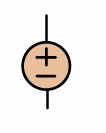
\includegraphics[width=\linewidth]{Images/Kapittel6:Elektrisitet/Spenningskilde(1).png}
        \caption{Spenningskilde 1}
        \label{fig:Spenningskilde1}
    \end{minipage}%
    \begin{minipage}{0.28\textwidth}
        \centering
        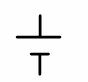
\includegraphics[width=\linewidth]{Images/Kapittel6:Elektrisitet/Spenningskilde(2).png}
        \caption{Spenningskilde 2}
        \label{fig:Spenningskilde2}
    \end{minipage}
\end{figure}



\textbf{Seriekobling}\\
En seriekobling er en krets som er koblet slik at strømmen bare kan gå "en vei". I Figur \ref{fig:Seriekobling} er R1, R2, og R3 resistanser og V1 er en spenningskilde. Strømmen vil gå inn og gjennom i R1, R2 og R3. Siden strømmen bare "har en vei" å gå, vil det i teorien være like mye strøm over hele området i seriekoblingen som vises i Figur \ref{fig:Seriekobling}. Strømmen har ingen plass å dele seg.

\begin{figure}[H]
    \centering
    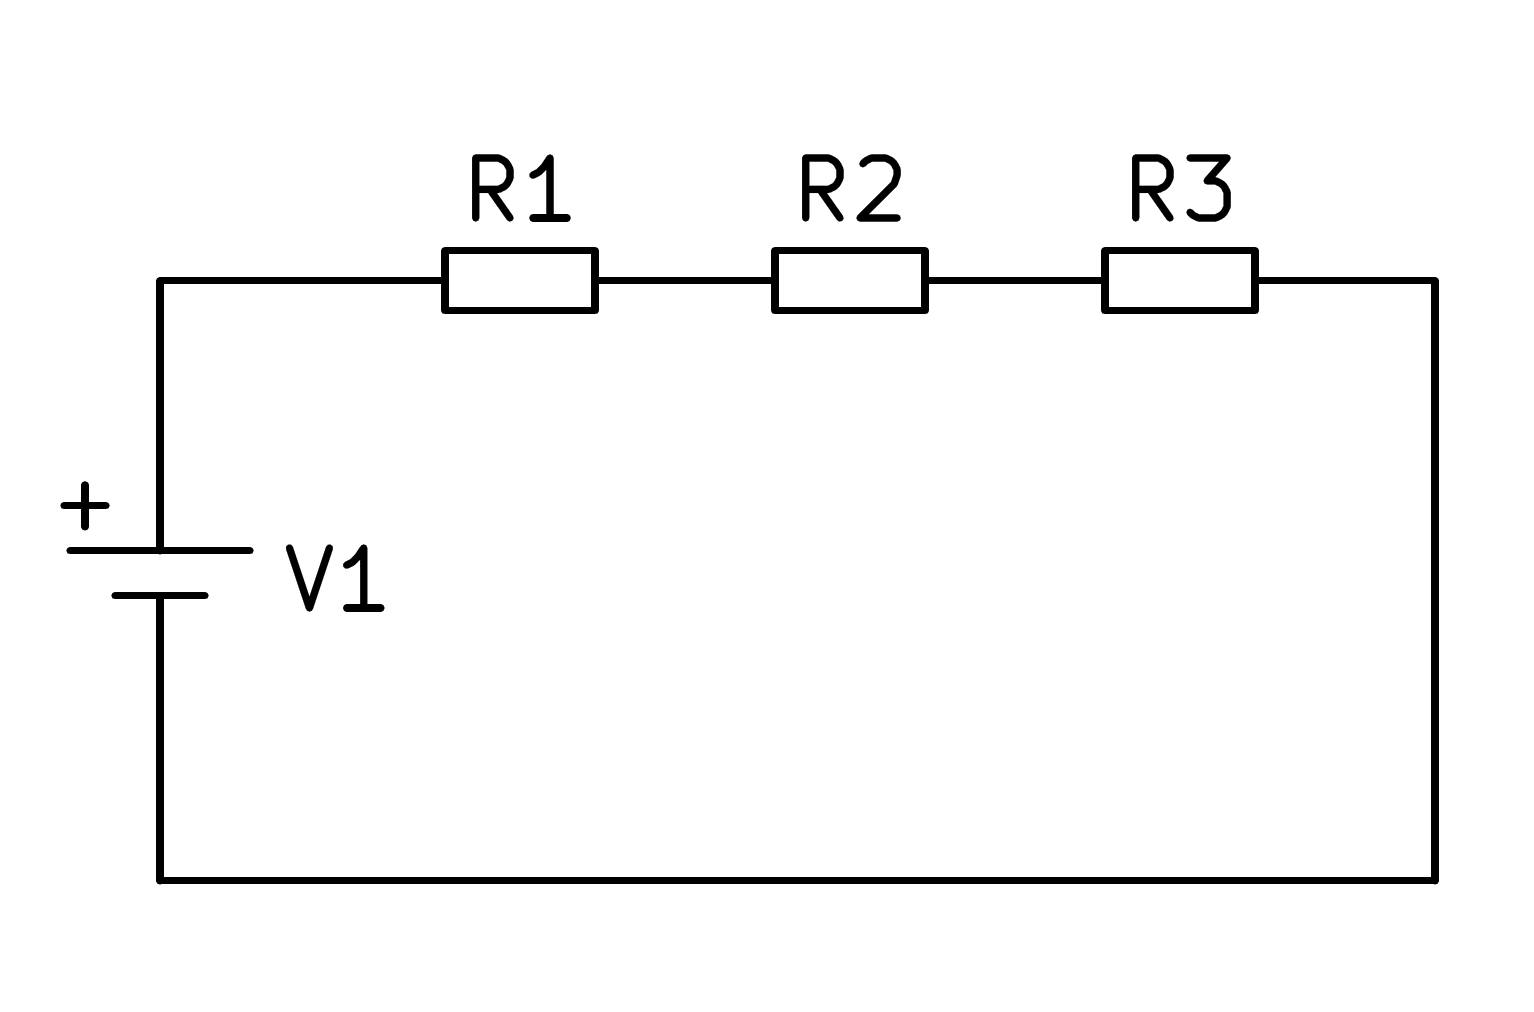
\includegraphics[width=0.5\textwidth]{Images/Kapittel6:Elektrisitet/Seriekobling.png}
    \caption{Seriekobling}
    \label{fig:Seriekobling}
\end{figure}


\textbf{Parallellkobling}\\
Parallellkobling er en måte å koble en krets slik at komponentene ligger "over" hverandre. I Figur \ref{fig:Parallellkobling} vises en parallellkobling, der R1 og R2 er resistanser og U er en spenningskilde. I denne kretsen vil strømmen vil gå fra spenningskilden og "dele" seg utover resistansene.\\
\begin{figure}[H]
    \centering
    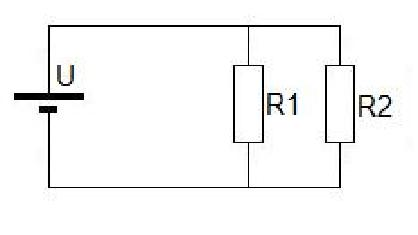
\includegraphics[width=0.5\textwidth]{Images/Kapittel6:Elektrisitet/Parallellkobling.png}
    \caption{Parallellkobling}
    \label{fig:Parallellkobling}
\end{figure}


\textbf{Leder, isolator og halvleder}\\
Stoffer deles inn i tre grupper etter evnen til å lede elektrisk strøm:
\begin{itemize}
  \item \textbf{Ledere} har mange løst bundne elektroner i det ytterste skallet.
        Disse kan bevege seg fritt og transportere ladning — metaller som kopper og aluminium er gode ledere.
  \item \textbf{Isolatorer} holder fast på alle elektroner; ingen kan bevege seg fritt.
        Eksempler: gummi, plast, glass. Brukes til å hindre strøm fra å renne «feil vei».
  \item \textbf{Halvledere} er midt imellom — ledningsevnen kan styres ved temperatur eller spenning.
        Grunnlaget for transistorer, dioder og all moderne elektronikk (silisium, Si).
\end{itemize}

\tips{Forståelse av elektroner, strøm og spenning}{Å forstå hva en elektrisk krets er og hvordan den fungerer kan være utfordrende. En god måte å tenke på en elektrisk krets er å forestille seg en krets bestående av elektroner som kuler plassert side om side. Disse elektronene kan bevege seg fra ett punkt til et annet innen kretsen. \\

Når en spenningskilde, som et batteri, påvirker elektronene nærmest seg, skaper dette en dominoeffekt der elektronene setter hverandre i bevegelse. En motstand kan ses på som en trangere del av kretsen, som gjør det vanskeligere for strømmen å passere, derav navnet "motstand". \\

I en \textbf{seriekobling} har elektronene bare én vei å følge gjennom kretsen. Denne veien forbinder ett punkt til et annet uten avkjøringer. \\


I en \textbf{parallellkobling}, derimot, deler veien seg og elektronene kan "velge" mellom flere stier. Dette resulterer i at strømmen tar veien med minst motstand på grunn av fysiske lover.}

\begin{figure}[H]
    \centering
    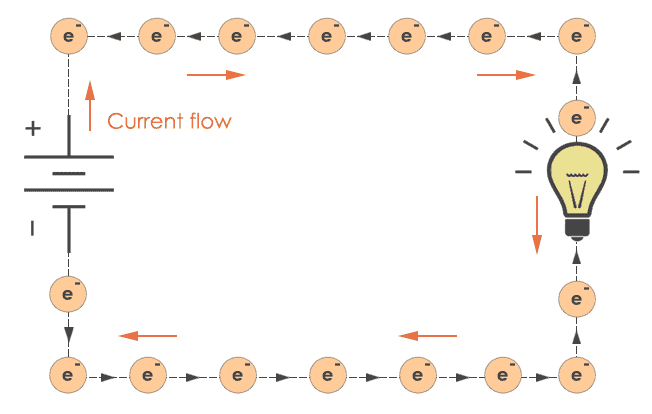
\includegraphics[width=0.5\linewidth]{Images/Kapittel6:Elektrisitet/Elektroner.png}
    \caption{Krets med elektroner i}
    \label{fig:Elektroner}
\end{figure}

%https://www.codrey.com/dc-circuits/conventional-current-vs-electron-current/   Hentet 31.12.2024



\section{Elektrisk kraft og ladning}

Elektrisk ladning er det som gir opphav til elektriske krefter.
To ladede legemer tiltrekker eller frastøter hverandre — akkurat som gravitasjon tiltrekker to masser,
men med en viktig forskjell: elektrisk kraft kan \emph{både} tiltrekke og frastøte.

\defn{Coulombs lov}{%
Kraften mellom to punktladninger $q_1$ og $q_2$ med avstand $r$ er:
\[
  F_e = k \frac{|q_1|\,|q_2|}{r^2}, \qquad k = \SI{8.99e9}{\newton\metre\squared\per\coulomb\squared}
\]
Kraften er \emph{tiltrekkende} dersom ladningene har motsatt fortegn, og \emph{frastøtende} dersom de har likt fortegn.
}

\begin{tcolorbox}[colback=gray!13, colframe=gray!40, boxrule=0.5pt,
    arc=2pt, left=6pt, right=6pt, top=4pt, bottom=4pt]
\textbf{Gravitasjon vs.\ elektrisitet — to naturkrefter med samme form}

\medskip
\begin{tabular}{lll}
  & \textbf{Gravitasjon} & \textbf{Elektrisitet} \\
  \hline
  Formel & $F_g = G\,\dfrac{m_1 m_2}{r^2}$ & $F_e = k\,\dfrac{|q_1||q_2|}{r^2}$ \\[8pt]
  «Ladning» & Masse $m$ & Elektrisk ladning $q$ \\
  Konstant & $G = \SI{6.67e-11}{}$ & $k = \SI{8.99e9}{}$ \\
  Retning & Alltid tiltrekkende & Tiltrekker (±) eller frastøter (++) \\
\end{tabular}

\medskip
Merk at $k$ er \emph{enorm} sammenliknet med $G$ — elektrisk kraft er typisk mange størrelsesordener sterkere enn gravitasjon på atomnivå.
\end{tcolorbox}

\exm{Kraft mellom to ladninger}{%
To ladninger $q_1 = \SI{+2.0}{\micro\coulomb}$ og $q_2 = \SI{-3.0}{\micro\coulomb}$
befinner seg $r = \SI{0.10}{\metre}$ fra hverandre.
Finn kraften mellom dem.

\[
  F_e = k\frac{|q_1||q_2|}{r^2}
      = \SI{8.99e9}{\newton\metre\squared\per\coulomb\squared}
        \cdot \frac{\SI{2.0e-6}{\coulomb}\cdot\SI{3.0e-6}{\coulomb}}{(\SI{0.10}{\metre})^2}
      = \doubleunderline{\SI{5.4}{\newton}}
\]
Siden ladningene har motsatt fortegn, er kraften \emph{tiltrekkende}.
}

\section{Kirchoff's lover}
Kirchoff's lover brukes til å regne ut strøm eller spenning i en elektrisk krets.

\subsection{Kirchoff's første lov}
Denne loven er også omtalt som \textit{Kirchoff's strømlov}. Denne loven går ut på at strømmen som går inn, eller ut av en node/knytepunkt til sammen blir 0.
\[\sum{I}=I_1+I_2+...+I_n=0\]

\subsection{Kirchoff's andre lov}
Denne loven er også omtalt som \textit{Kirchoff's spenningslov}.

\[\sum{U}=U_1+U_2+...+U_n=0\]



\subsection{Fysisk tolkning}

\textbf{Kirchhoffs 1.\ lov} (strømloven) følger av at ladning er bevart: ingen ladning kan «forsvinne» i et forgreningspunkt, så all strøm inn må ut igjen.

\textbf{Kirchhoffs 2.\ lov} (spenningsloven) følger av energibevaring: i en lukket sløyfe må summen av alle spenningsfall (over motstander) være lik summen av alle spenningsstigninger (fra kilder). Tilsvarende: vandrer du i en ring tilbake til startpunktet, er nettohøydeforskjellen null.

\exm{Krets med Kirchhoffs lover}{%
En krets har en spenningskilde $U_0 = \SI{24}{\volt}$.
Motstand $R_1 = \SI{3}{\ohm}$ er i serie med en parallellkobling av $R_2 = \SI{6}{\ohm}$ og $R_3 = \SI{12}{\ohm}$.

\begin{center}
\begin{tikzpicture}[scale=0.92, >={Stealth[length=4pt,width=3pt]},
    component/.style={draw, thick, minimum width=0.5cm, minimum height=0.9cm}]
  % Nodes
  \coordinate (A) at (0,2);
  \coordinate (B) at (3,2);
  \coordinate (C) at (5,2);
  \coordinate (D) at (5,0);
  \coordinate (E) at (3,0);
  \coordinate (F) at (0,0);
  % Battery
  \draw[thick] (A) -- (F);
  \draw[thick] (0,1.3) -- (0,0.7);
  \node[left, font=\footnotesize] at (-0.1,1.0) {$U_0$};
  \draw[thick, double] (0,1.15) -- (0,0.85);
  % Top wire
  \draw[thick] (A) -- (B);
  % R1
  \draw[thick] (B) -- (B)+(0.3,0);
  \draw[thick, decorate, decoration={zigzag,segment length=4pt,amplitude=3pt}]
      (3.3,2) -- (4.7,2);
  \node[above, font=\footnotesize] at (4,2.3) {$R_1$};
  \draw[thick] (4.7,2) -- (C);
  % Junction C
  \fill (C) circle (0.06);
  % R2 (upper branch)
  \draw[thick] (C) -- (5,2.7);
  \draw[thick, decorate, decoration={zigzag,segment length=4pt,amplitude=3pt}]
      (5,2.7) -- (5,3.5);
  \node[right, font=\footnotesize] at (5.2,3.1) {$R_2$};
  \draw[thick] (5,3.5) -- (3,3.5) -- (E);
  % R3 (lower branch)
  \draw[thick] (C) -- (5,1.3);
  \draw[thick, decorate, decoration={zigzag,segment length=4pt,amplitude=3pt}]
      (5,1.3) -- (5,0.5);
  \node[right, font=\footnotesize] at (5.2,0.9) {$R_3$};
  \draw[thick] (5,0.5) -- (D);
  % Bottom wire
  \fill (E) circle (0.06);
  \draw[thick] (E) -- (F);
  % Current labels
  \node[above, font=\footnotesize, defscol] at (1.5,2) {$I_0$};
  \node[right, font=\footnotesize, headCol] at (5.5,3.1) {$I_2$};
  \node[right, font=\footnotesize, headCol!60!black] at (5.5,0.9) {$I_3$};
\end{tikzpicture}
\end{center}

\noindent\textbf{Steg 1 — Totalmotstand:}

Parallellkoblingen: $\frac{1}{R_p} = \frac{1}{6} + \frac{1}{12} = \frac{3}{12}$,
så $R_p = \SI{4}{\ohm}$.

Totalmotstanden: $R_{\text{tot}} = R_1 + R_p = 3 + 4 = \SI{7}{\ohm}$.

\noindent\textbf{Steg 2 — Totalstrøm (Kirchhoffs 2.\ lov + Ohms lov):}
\[
  U_0 = R_{\text{tot}}\,I_0 \implies I_0 = \frac{U_0}{R_{\text{tot}}} = \frac{\SI{24}{\volt}}{\SI{7}{\ohm}}
  \approx \doubleunderline{\SI{3.43}{\ampere}}
\]

\noindent\textbf{Steg 3 — Spenning over parallellkoblingen:}
\[
  U_p = R_p\,I_0 = \SI{4}{\ohm}\cdot\SI{3.43}{\ampere} \approx \SI{13.7}{\volt}
\]

\noindent\textbf{Steg 4 — Strøm i grenene (Kirchhoffs 1.\ lov):}
\[
  I_2 = \frac{U_p}{R_2} = \frac{13.7}{6} \approx \SI{2.29}{\ampere}, \qquad
  I_3 = \frac{U_p}{R_3} = \frac{13.7}{12} \approx \SI{1.14}{\ampere}
\]
Sjekk K1: $I_2 + I_3 \approx 2.29 + 1.14 = \SI{3.43}{\ampere} = I_0$ \checkmark
}

\section{Motstand}
Motstand, eller resistanser, R, er komponenter i en krets som har påvirkning på strømmen og spenningen. \textit{Ohm's lov} viser at spenningen, U, er proporsjonal med resistansen og strømmen. 

\defn{Ohm's lov}{\centering U=R$\cdot$ I \\
Hvor U er spenningen i volt, \textit{V}, R er resistansen i ohm \textit{$\Omega$} og I er strømmen i ampere, \textit{A}.}

Ohm's lov viser at strømmen, I$=$$\frac{U}{R}$, er er omvendt proporsjonal med resistansen. Det vil si at det høyere motstand, det mindre strøm vil gå. Ved fullstendig motstand, for eksempel ved en åpen krets, er det teoretisk sett ingen strøm som passerer. Ved mindre motstand, er det lettere for strømmen å gå.

\subsection{Motstander i seriekobling}
Når motstander er seriekoblet, kan man finne den totale motstanden i kretsen ved bruk av Formel \ref{eq:sum_motstand_serie}.

\begin{align}
    &\sum R_{tot}= R_1+R_2 +...+ R_n
    \label{eq:sum_motstand_serie}
\end{align}


\exm{Sum av motstand i seriekobling}{De to øverste i Figur \ref{fig:Seriekobling_motstand} mostandende er henholdsvis 6$\Omega$ og 10$\Omega$. Hvis summen av motstander i kretsen er 25 $\Omega$, hva er da verdien til den siste motstanden? \\
Bruker formelen:\\
\[\ R_{tot}=R_1+R_2+R_3\]\\
\[\ R_3=R_{tot}-R_1-R_2\]}


\begin{figure}[H]
    \centering
    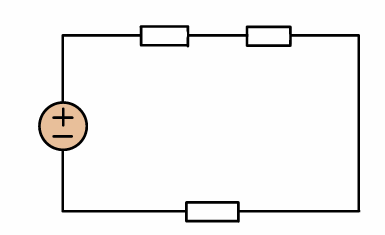
\includegraphics[width=0.3\linewidth]{Images/Kapittel6:Elektrisitet/Krets_med_spenningskilde(1).png}
    \caption{Motstander i seriekobling}
    \label{fig:Seriekobling_motstand}
\end{figure}




\subsection{Motstander i parallellkobling}
Når motstander ligger i parallellkobling, kan man finne den totale motstanden i kretsen ved bruk av Formel \ref{eq:sum_motstand_parallell}.
\begin{align}
    &\sum \frac{1}{R_{tot}}= \frac{1}{R_1} + \frac{1}{R_2} +...+ \frac{1}{R_n}
    \label{eq:sum_motstand_parallell}
\end{align}

\begin{figure}[H]
    \centering
    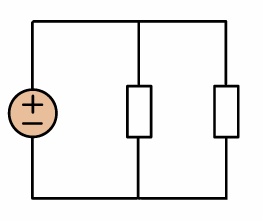
\includegraphics[width=0.3\linewidth]{Images/Kapittel6:Elektrisitet/Parallellkobling_motstander.png}
    \caption{Motstander i parallellkobling}
    \label{fig:Parallellkobling_motstander}
\end{figure}


\subsection{Elektrisk strøm og ladning}
Elektrisk strøm er definert som elektrisk ladning i bevegelse. Det finnes \textit{vekselstrøm} og \textit{likestrøm}. Vekselstrøm er strøm med varierende retning, mens likestrøm har samme retning. Strømmen i stikkontakten som er knyttet opp mot strømnettet er vekselstrøm. I TRES skal det være fokus på likestrøm. Likestrøm får man fra for eksempel batterier, hvor strømmen går i en retning. Elektronene går fra negativ pol til positiv pol i en lukket krets. En \textit{lukket krets} er en krets som er koblet sammen på begge sider av batteri og komponenter. En \textit{åpen krets} er en krets som har et "hull" i seg, eller som ikke er koblet opp på både positiv og negativ pol.



\subsubsection{Elementærladning}
Elementærladningen er den elektriske ladningen til et proton. Elektroner har samme størrelse på ladning som protoner, bare i motsatt retning. Derfor er ladningen til et elektron lik \textit{-e}. \\
\[e=1,602 \cdot 10^{-19} C\]

\defn{Strøm og ladning}{Nedenfor står en formel for strøm, hvor \textit{I} er strøm i Ampere, \textit{q} er ladning i Coulomb og \textit{t} er tid i sekund.\\
\centering I=$\frac{q}{t}$ \\
Under står en formel for ladningen \textit{q}, elementærladningen er \textit{e}=1,602$\cdot$ 10$^{-19}$ C og \textit{N} er antall elektroner. \\
\centering q=e$\cdot$N\\
}

\exm{Antall elektroner}{Ladningen på et område er -100 Coulomb. Hvor mange overskudds-elektroner er på området? \\
\[q=e\cdot N\]
\[N=\frac{q}{e}\]
\[N=\frac{-100 C}{-1,602\cdot 10^{-19}\frac{C}{elektroner}}\]
\[N=6,24\cdot 10^{20} elektroner\]}


\section{Effekt}
Effekt innenfor elektrisitet er elektrisk energi per tidsenhet. Effekten er proporsjonal med strømmen og spenningen.

\defn{Effekt}{Nedenfor står formelen for effekt, \textit{P}. \textit{U} er spenningen og \textit{I} er strømmen.
\[P=U\cdot I\]
Spenningen kan regnes ved:
\[U=R\cdot I\]
Dermed kan effekten også skrives som:
\[P=R\cdot I^2\]
}

\subsection{Eksempeloppgaver}

\tips{Hvordan løse oppgaver innen for elektrisitet?}{Steg for steg over hvordan løse oppgaver innenfor elektrisitet:

\begin{enumerate}
    \item \textbf{Tegn kretsen} - Start med å visualisere problemet ved å tegne kretsen. Dette gir en klar oversikt og hjelper deg å identifisere hvilke komponenter som er involvert.

    \item \textbf{Identifiser koblingstype} - Bestem om kretsen består av en seriekobling, parallellkobling eller en kombinasjon av begge. Dette påvirker hvordan strøm og spenning distribueres gjennom kretsen.

    \item \textbf{Forenkel kretsen} - Bruk prinsippene vist i eksemplene i dette kapittelet for å forenkle kretsen til mer håndterbare deler. Dette kan inkludere å kombinere resistanser i serie eller parallell for å redusere kompleksiteten.

    \item \textbf{Løs oppgaven med relevante formler} - Etter at du har forenklet kretsen, bruk relevante elektriske formler for å finne de ønskede verdier som strøm, spenning eller motstand. Sørg for å lese oppgaveteksten nøye for å forstå hva som er spurt om.
\end{enumerate}}


\exm{Krets 1}{Krets 1 består av et batteri som energikilde, med en spenning på 5 V. Batteriet er seriekoblet med spenningen R$_1$. R$_1$ er koblet opp med to resistanser i seriekobling R$_2$ og R$_3$. R$_1$ er på 1 $\Omega$, R$_2$ er på 2 $\Omega$, mens R$_3$ er på 1,4 $\Omega$.

a) Hva er den totale strømmen i kretsen?

Løsning:
1. \textbf{Tegn kretsen.} Se Figur \ref{fig:parallellkobling_eksempel} som eksempel på en tegning.\\

2. \textbf{Identifiser koblingstype}. R$_1$ er i serie med R$_2$ og R$_3$ i parallellkobling.\\

3 \textbf{Forenkle kretsen.} Første steg her er å "sette sammen" R$_2$ og R$_3$ slik at de representerer en resistans. Formel \ref{eq:sum_motstand_parallell} viser hvordan det kan regnes ut.

\[\Sigma R_{parallell} = (\frac{1}{R_2}+\frac{1}{R_3})^{-1}\]
\[\Sigma R_{parallell} = (\frac{1}{2}+\frac{1}{1,4})^{-1}\]
\[\Sigma R_{parallell} = 0,82 \Omega\]

4. \textbf{Løs oppgaven med relevante formler.} Kretsen består nå av batteriet koblet opp med to resistanser, R$_1$ og R$_{paralell}$. Den totale resistansen blir da, ved hjelp av formel for seriekoblet resistanser; Formel \ref{eq:sum_motstand_serie}:

\[\Sigma R_{serie} = \Sigma R_{total} =1 + 0,82\]
\[\Sigma R_{serie} = 1,82\]

Da blir strømmen 2,74. Det fant vi ved bruk av U=RI.}



\begin{figure}[H]
    \centering
    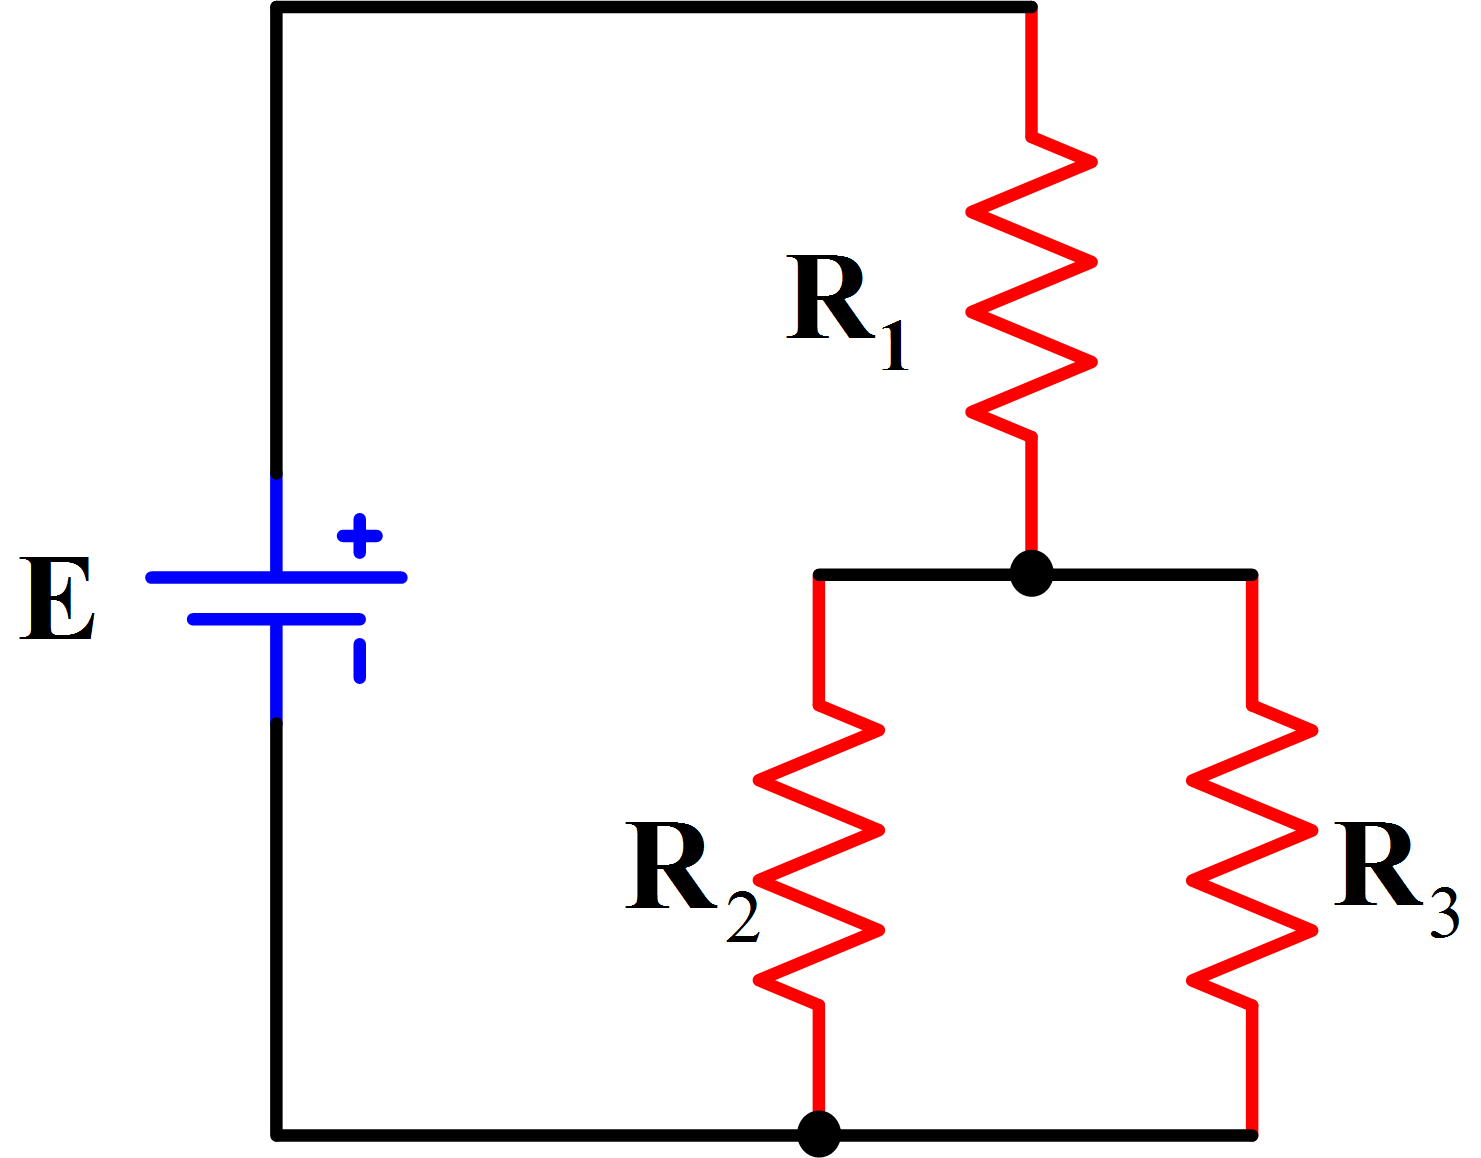
\includegraphics[width=0.5\linewidth]{Images/Kapittel6:Elektrisitet/Parallellkobling_eksempel.png}
    \caption{Tegning av Krets 1}
    \label{fig:parallellkobling_eksempel}
\end{figure}